\chapter{Towards studies of correlation effects in attosecond electron dynamics} % (fold)
\label{cha:electron_correlation}


Solving the TDSE for two active electrons is a computationally difficult task. A naive approach would be to discretize the six spatial dimensions using finite difference. This approach would provide a straightforward solution and runs well on supercomputing systems, however, the size of the wavefunction scales like $N^6$ where $N$ is the number of grid points in each dimension. Therefore, if one were to use a typical grid of 1000 points in each dimension, the wavefunction would be $10^{18}$ points in size. Merely writing down the wavefunction in double precision floating point numbers would require 16 Exabytes of RAM, approximately 100 times more RAM than exists on the largest supercomputer in the world (Summit, Oak Ridge Leadership Computing Facility). Instead, it is more convenient to choose a coordinate system and basis that greatly reduces the size of the problem. One common approach is to use bi-spherical harmonics (e.g. \cite{vanroose2006}). In this case, the position of each electron is expanded in 3D spherical coordinates. The radius is discretized with finite difference, B-splines, finite-element discrete variable representation (FEDVR), or similar method, and the two angular coordinates are expanded in the standard 3D spherical harmonics in the same way a single active electron code would do. When taking the tensor product of the two electrons, the electron-electron repulsion term is then expanded in spherical harmonics such that
\begin{equation}
    \frac{1}{|\mathbf{r}_1-\mathbf{r}_2|}= 4\pi \sum_{\ell=0}^\infty \sum_{m=-\ell}^{m=\ell}\frac{1}{2\ell+1}\frac{r_<^\ell}{r_>^{\ell+1}}Y_{\ell m}^*(\theta_1, \phi_1)Y_{\ell m}(\theta_2, \phi_2).
\end{equation}
This results in a representation of the 6D space that can be used to solve the problem of two electrons in a molecular or atomic potential interacting with a laser.

In the bi-spherical codes, one must discretize two radii. As the grid increases in size, the code still scales like $N^2$. To circumvent this problem, we have implemented a code that contains a single hyper-radius ($R$) and five angles that are expanded in 6D hyperspherical harmonics. Therefore, as the grid size is increased, the code scales like $N$ and the number of spherical harmonics is controlled by the laser parameters. In the following section, we will describe the details to utilize two different ``coordinate systems'' that solve the two active electron problem. The first is based on the use of Jacobi coordinates, which allows for the finite mass of the nucleus to be accounted for. The second is applied when using the infinite mass approximation for the nucleus, which allows that the distance between the two electrons to be accessed more directly. The two problems can be solved with similar sized wavefunctions, however, the time to calculate matrix elements is greatly reduced in the second method. 

This chapter covers the background for the TDSE program developed in hyperspherical coordinates in Sec.~\ref{sec:tdse_in_hyperspherical_coordinates} including the definition of hyperspherical harmonics in Sec.~\ref{sub:spherical_harmonics}, the application of Jacobi coordinates in Sec.~\ref{sub:jacobi_coordinates}, and the application of electron coordinates in Sec.~\ref{sub:jacobi_coordinates}. A discussion of the implementation of the code and first tests will be presented in Sec.~\ref{sec:implementation_and_first_tests} while Sec.~\ref{sec:outlook} provides a brief overview of the challenges that remain and useful next steps which will make it possible to run fully correlated two-electron calculations on desktop machines.

\section{TDSE in hyperspherical coordinates} % (fold)
\label{sec:tdse_in_hyperspherical_coordinates}
The TDSE
\begin{equation}
    i\frac{\partial}{\partial t}\Psi = \hat{H}\Psi
\end{equation}
with Hamiltonian written in hyperspherical coordinates is given by
\begin{equation}
   \hat{H} = -\frac{1}{2} \left[\frac{1}{R^5}\frac{\partial}{\partial R}\left(R^5\frac{\partial}{\partial R}\right) - \frac{\hat{K}^2(\Omega_5)}{R^2}\right] + \frac{W(\Omega_5)}{R}\, ,
\end{equation}
where $R=\sqrt{\sum_i x_i^2}$ is the hyperradius with $x_i$ being a Cartesian coordinate, $\hat{K}$ is the angular momentum operator, $\Omega_5$ is the solid angle in 6D (5 angles), and $V(\mathbf{R}) = W(\Omega_5)/R$ being the potential. We will use the hyperspherical harmonics which contain two-3D sub spaces as described in Sec.~\ref{sub:spherical_harmonics}. 
The resulting volume elements are 
\begin{equation}
    d\tau = R^5 dr d\Omega_5
\end{equation}
\begin{equation}
    d\Omega_5 = \cos^2\alpha \sin^2\alpha d\alpha d\omega
\end{equation}
\begin{equation}
    d\omega = \sin\theta_\mathbf{r_1} d\theta_\mathbf{r_1} d\phi_\mathbf{r_1} \sin\theta_\mathbf{r_2} d\theta_\mathbf{r_2} d\phi_\mathbf{r_2}
\end{equation}
where $\theta_i$ and $\phi_i$ denote the angles in the $i=\mathbf{r_1}$ and $i=\mathbf{r_2}$ sub coordinate systems and $\alpha$ is the angle produced by the right triangle with sides $R$, ${r_1}$, and ${r_2}$ as shown in Fig.~\ref{fig:hyperradius}. $r_1$ and $r_2$ will denote the Jacobi Coordinates, if a finite mass nucleus is considered, or the single electron coordinates when the infinite mass approximation is made.
\begin{figure}[h!]
\centering
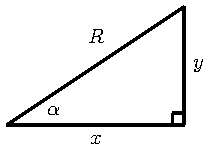
\includegraphics[width=0.3\linewidth]{figs/Two_electron/hyperradius.pdf}
\caption{Relation of the hyperradius ($R$) to the two single-electron sub coordinate systems ($r_1$, $r_2$).} 
  \label{fig:hyperradius}
\end{figure}

As for the 3D TDSE, it is beneficial to remove the first derivative in the radial equation. This is accomplished by substituting $\Psi = \psi/R^{5/2}$ to get as Hamiltonian
\begin{equation}
   \hat{H} = -\frac{1}{2} \left[\frac{\partial^2}{\partial R^2} - \frac{\hat{K}^2(\Omega_5)+15/4}{R^2}\right] + \frac{W(\Omega_5)}{R}.
\end{equation}
The wavefunction can now be written as
\begin{equation}
    \psi = \sum\limits_{\mathbf{K}} U_{\mathbf{K}}(R) Y_{\mathbf{K}}(\Omega_5)
\end{equation}
with $U_{\mathbf{K}}(R)$ being the hyperradial part of the wavefunction and $Y_{\mathbf{K}}(\Omega_5)$ being the 6D hyperspherical harmonics described in Sec.~\ref{sub:spherical_harmonics}. Since hyperspherical harmonics are eigenfunctions of $\hat{K}^2$ with eigenvalue $K(K+4)$, the Hamiltonian becomes
\begin{equation}
   \hat{H}_{K} = -\frac{1}{2} \left[\frac{\partial^2}{\partial R^2} - \frac{K(K+4)+15/4}{R^2}\right] + \frac{W(\Omega_5)}{R}.
\end{equation}
We solve this equation using finite difference to discretize the hyperradial function $U_{\mathbf{K}}(R)$. For $W(\Omega_5)=1$ the equation is the 6D hydrogen atom (i.e. an electron interacting with a Coulomb potential in 6 spacial dimensions, rather than the typical 3 spacial dimension) with an analytic solution that can be used to test the hyperadial portion of the code (see \cite{sorevik2005} for energy levels). The angular portion of the equations is then expanded in hyperspherical harmonics. The details of the expansion are the focus of the remainder of this section.
% subsection tdse_in_hyperspherical_coordinates (end)

\subsection{Hyperspherical harmonic definition} % (fold)
\label{sub:spherical_harmonics}
There are multiple ways to define hyperspherical harmonics in 6D. Since they are equivalent up to a unitary rotation, it is best to choose those that match the symmetry of the problem. In our case, we choose spherical harmonics that contain a hyperangle $\alpha$ that connects two-3D spaces as shown in Fig.~\ref{fig:hyperradius}. The 3D spaces belong to coordinates $\mathbf{r}_1$ and $\mathbf{r}_2$ with radii $r_1$ and $r_2$ respectively. These spaces will either represent a Jacobi coordinate (Sec.~\ref{sub:jacobi_coordinates}) or the space of each electron (Sec.~\ref{sub:electronic_coordinates}). The resulting 6D spherical harmonics are given by
\begin{align}
    Y^{\ell_{r_1},\ell_{r_2}}_{K,L,M}(\Omega_{5}) =& N^{\ell_{r_1},\ell_{r_2}}_K P_n^{(\ell_{r_1}+1/2,\ell_{r_2}+1/2)}(\cos(2\alpha)) \cos^{\ell_{r_1}}(\alpha) \sin^{\ell_{r_2}}(\alpha) \\ 
    &\times\sum_{m_{r_1},m_{r_2}}\bra{L,M}\ket{\ell_{r_1},m_{r_1},\ell_{r_2},m_{r_2}}  \left[Y_{\ell_{r_1},m_{r_1}}(\hat{r}_1) Y_{\ell_{r_2},m_{r_2}}(\hat{r}_2)\right]
\end{align}
with
\begin{equation}
    N^{\ell_{r_1},\ell_{r_2}}_K = \sqrt{\frac{2(K+2)(n!)\Gamma (n+\ell_{r_1}+\ell_{r_2}+2)}{\Gamma (n+\ell_{r_1}+3/2) \Gamma (n+\ell_{r_2}++3/2)}}.
\end{equation}
where $P_n^{(\alpha,\beta)}$ is the Jacobi polynomial,  $\bra{L,M}\ket{\ell_{r_1},m_x,\ell_{y_1},m_y}$ is a Clebsch–Gordan coefficient (CGC), $\Gamma$ is the gamma function, $Y_{\ell_{r},m_{r}}(\hat{r})$ is the standard 3D spherical harmonics, $\Omega_5$ is the 6D solid angle containing five angular dimensions, and $n = (K-\ell_{x_1}-\ell_{y_1})/2$. $K$, $L$, $M$, $\ell_{r_1}$ and $\ell_{r_2}$ are the quantum numbers with $K=2n+\ell_{x_1}+\ell_{y_1}$ being the grand angular momentum, $\ell_{r_1}\ge0$ and $\ell_{r_2}\ge0$ being the angular momentum for the $\mathbf{r}_1$ and $\mathbf{r}_2$ coordinates, respectively, $|\ell_{r_1}-\ell_{r_2}|\le L \le \ell_{r_1}+\ell_{r_2}$ and $-L \le M \le L$. We define $\mathbf{K}=\{K, L, M, \ell_{r_1}, \ell_{r_2}\}$ allowing for the simplified notation $Y_{\mathbf{K}}(\Omega_{5})$.

The hyperspherical harmonics contain three parts, each depending on one free parameter $\alpha$, $\mathbf{r}_1$, and $\mathbf{r}_2$. By defining 
\begin{equation}
    \tilde{P}^{\ell_{r_1},\ell_{r_2}}_{n}(\alpha) = N^{\ell_{r_1},\ell_{r_2}}_K P_n^{(\ell_{r_1}+1/2,\ell_{r_2}+1/2)}(\cos(2\alpha)) \cos^{\ell_{r_1}}(\alpha) \sin^{\ell_{r_2}}(\alpha) 
\end{equation}
hyperspherical harmonics become
\begin{equation}
    Y^{\ell_{r_1},\ell_{r_2}}_{K,L,M}(\Omega_{5}) =\tilde{P}^{\ell_{r_1},\ell_{r_2}}_{n}(\alpha)\sum_{m_{r_1},m_{r_2}}\bra{L,M}\ket{\ell_{r_1},m_{r_1},\ell_{r_2},m_{r_2}}  \left[Y_{\ell_{r_1},m_{r_1}}(\hat{r}_1) Y_{\ell_{r_2},m_{r_2}}(\hat{r}_2)\right]\, ,
    \label{eq:hyperspherical_harm_simple}
\end{equation}
which highlights the three main components including the dependence of the angles in the spaces $r_1$ and $r_2$ as well as the dependence on the hyperangle $\alpha$ that couples the two spaces.
% section spherical_harmonics (end)
 
\subsection{Jacobi coordinates} % (fold)
\label{sub:jacobi_coordinates}
Jacobi coordinates are often used for studying many body interactions. They are defined by choosing a particle and defining a relative coordinate between the chosen particle and a second particle. The next particle is defined by a coordinate connecting the center of mass of all the previous particles to the new particle. The pattern continues until all particles have been included. The result is a set of coordinates that has dimension $3(N-1)$ assuming the exact location of the center of mass $R_{cm}$ in space is irrelevant. 
For a three particle system, the center of mass is given by
\begin{equation}
\mathbf{R}_{cm} = \frac{m_1 \mathbf{r}_1 + m_2 \mathbf{r}_2 + m_3 \mathbf{r}_3}{M}
\end{equation}
with $m_i$ being the mass of the $ith$ particle, $\mathbf{r}_i$ being its spatial coordinate, and $M = \sum_{i=1}^3m_i$.
The three convenient sets of Jacobi coordinates are
\begin{align}
\label{eq:jacobi_coords}
\mathbf{x}_1 &= \left[\frac{m_2m_3M}{m_1(m_2+m_3)^2}\right]^{1/4} (\mathbf{r}_3-\mathbf{r}_2); &\mathbf{y}_1 &= \left[\frac{m_1(m_2+m_3)^2}{m_2m_3M}\right]^{1/4} \left(\mathbf{r}_1- \frac{m_2\mathbf{r}_2+m_3\mathbf{r}_3}{m_2+m_3} \right)\\
\mathbf{x}_2 &= \left[\frac{m_3m_1M}{m_2(m_3+m_1)^2}\right]^{1/4} (\mathbf{r}_1-\mathbf{r}_3); &\mathbf{y}_2 &= \left[\frac{m_2(m_3+m_1)^2}{m_3m_1M}\right]^{1/4} \left(\mathbf{r}_2- \frac{m_3\mathbf{r}_3+m_1\mathbf{r}_1}{m_3+m_1} \right)\\
\mathbf{x}_3 &= \left[\frac{m_1m_2M}{m_3(m_1+m_2)^2}\right]^{1/4} (\mathbf{r}_2-\mathbf{r}_1); &\mathbf{y_3} &= \left[\frac{m_3(m_1+m_2)^2}{m_1m_2M}\right]^{1/4} \left(\mathbf{r}_3- \frac{m_1\mathbf{r}_1+m_2\mathbf{r}_2}{m_1+m_2} \right).
\end{align}
The three coordinate systems are depicted in Fig.~\ref{fig:jacobi_coord}. For the Helium atom we choose the nucleus as $m_1$ and the two electrons as $m_2$ and $m_3$. For the rest of the section, we set $m_1\rightarrow \infty$ and $m_2=m_3=m$ such that
\begin{align}
\mathbf{x}_1 &= \beta_1 (\mathbf{r}_3-\mathbf{r}_2); \; \; \mathbf{y}_1 = \frac{1}{\beta_1} \left(\mathbf{r}_1- \frac{\mathbf{r}_2+\mathbf{r}_3}{2} \right)\\
\mathbf{x}_2 &= \beta_2 (\mathbf{r}_1-\mathbf{r}_3); \; \; \mathbf{y}_2 = \frac{1}{\beta_2} \left(\mathbf{r}_2- \frac{\mathbf{r}_3+\mathbf{r}_1}{2} \right)\\
\mathbf{x}_3 &= \beta_3 (\mathbf{r}_2-\mathbf{r}_1); \; \; \mathbf{y}_3 = \frac{1}{\beta_3} \left(\mathbf{r}_3- \frac{\mathbf{r}_1+\mathbf{r}_2}{2} \right)\, ,
\end{align}
where $\beta_1=1/\sqrt{2}$ and $\beta_2=\beta_3=1$ within the infinite mass approximation. By applying a Raynal-Revai coefficient (RRC) it is possible to transition between the three different coordinate systems.  The transformation conserves the angular momentum quantum numbers $K$, $L$, and $M$ of the hyperspherical harmonics.

\begin{figure}[!ht]
\centering
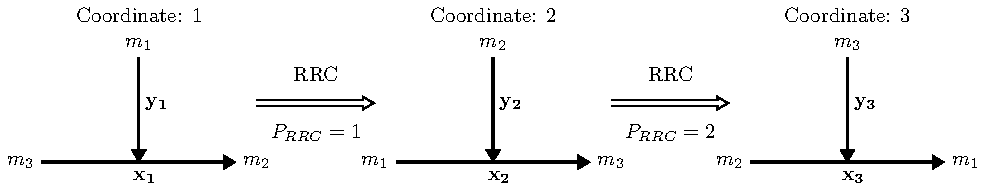
\includegraphics[width=\linewidth]{figs/Two_electron/coord_1.pdf}
\caption{The Jacobi coordinates for three body interactions. Each coordinate can be obtained from the previous by utilizing a Raynal-Revai coefficient.} 
  \label{fig:jacobi_coord}
\end{figure}

The RRCs for rotating between coordinate system $i$ and $j$ can be written explicitly as
\begin{align}
\nonumber
    <\ell_{x_j},\ell_{y_j}|\ell_{x_i},\ell_{y_i}>_{K,L} =& \frac{(-1)^{n_i+n_j}}{\sqrt{C_{\ell_{x_j}\ell_{y_j}}^{n_j}C_{\ell_{x_i}\ell_{y_i}}^{n_i}}} \sum\limits_{\lambda_1,\lambda_2,\lambda_3,\lambda_4} i^{\lambda_2-\lambda_1+\ell_{y_i}-\ell_{y_j}}\left[\prod_{k=1}^4 (2\lambda_k +1)\right] \\ 
\nonumber
    & \times \braket{\lambda_1 0 \lambda_3 0}{\ell_{x_j} 0} \braket{\lambda_2 0 \lambda_3 0}{\ell_{x_i} 0} \braket{\lambda_2 0 \lambda_4 0}{\ell_{y_j} 0} \braket{\lambda_1 0 \lambda_4 0}{\ell_{y_i} 0} \\
\nonumber
    & \times \sgn(a_{12})^{\lambda_1}\sgn(a_{21})^{\lambda_2}\sgn(a_{11})^{\lambda_3}\sgn(a_{22})^{\lambda_4} \begin{bmatrix}
  \lambda_3 & \lambda_1 & \ell_{x_j} \\
  \lambda_2 & \lambda_4 & \ell_{y_j} \\
  l_{x_i}   & l_{y_i}   & L
  \end{bmatrix} \\
    & \times \sum\limits_{\nu,\mu} (-1)^{\mu}|a_{12}|^{2\mu + \lambda_1 + \lambda_2} |a_{12}|^{2\nu + \lambda_3 + \lambda_4} C_{\lambda_1 \lambda_2}^{\mu} C_{\lambda_3 \lambda_4}^{\nu}
    \label{eq:RRC}
\end{align}
where $\sgn(a_{ij})$ is the sign of $a_{ij}$, between spherical harmonics with quantum numbers $K=2n_i+\ell_{x_i}+\ell_{y_i}=2n_j+\ell_{x_j}+\ell_{y_j}$, the sums go over all possible combinations of $K=2(\mu+\nu)+\lambda_1+\lambda_2+\lambda_3+\lambda_4$ with $(\lambda_i, \mu, \nu = 0,1,2,\cdots)$, $\braket{\lambda_1 0 \lambda_3 0}{\ell_{x_j} 0}$ is a Clebsch Gordan coefficient,
     $\begin{bmatrix}
        \lambda_3 & \lambda_1 & \ell_{x_j} \\
        \lambda_2 & \lambda_4 & \ell_{y_j} \\
        l_{x_i}   & l_{x_y}   & L
        \end{bmatrix}$
is a Wigner 9j symbol, 
    $C_{\alpha\beta}^\mu = \frac{(2\mu+\alpha+\beta+1)!}{(\mu)!(\mu+\alpha+\beta+1)!(2(\mu+\alpha)+1)!!(2(\mu+\beta)+1)!!}$,
$a_{11} = \cos(\xi_{ki})$,
$a_{22} = \cos(\xi_{ki})$,
$a_{12} = \sin(\xi_{ki})$, and 
$a_{21} = -\sin(\xi_{ki})$
with $\xi_{ki} = \arctan((-1)^{P_{RRC}}\sqrt{Mm_j/(m_i m_k)})$ where $m_i$ is the mass of the $i$th particle, $M$ is the total mass and $P$ is the number of permutations of $m_1\rightarrow m_2\rightarrow m_3\rightarrow m_1$  as shown in Fig.~\ref{fig:jacobi_coord}. As the value of $K$ increases, RRCs become extremely computationally expensive limiting the usefulness of this approach.


Utilizing the Jacobi coordinates, denoted by `1' in Fig.~\ref{fig:jacobi_coord}, the Helium potential becomes
\begin{equation}
    V(\mathbf{R}) = \frac{1}{r_{23}} - \frac{Z}{r_{12}} - \frac{Z}{r_{13}}
\end{equation}
which can be rewritten as 
\begin{equation}
    W(\Omega_5) = R V(\mathbf{R}) = \frac{1}{x_1\sqrt{2}} - \frac{Z\sqrt{2}}{|\hat{y}_1+\hat{x}_1|} - \frac{Z\sqrt{2}}{|\hat{y}_1-\hat{x}_1|}.
\end{equation}
By using the hyperspherical harmonics defined in Eq.~\ref{eq:hyperspherical_harm_simple}, with $\mathbf{r}_1=\mathbf{x}_1$ and $\mathbf{r}_2=\mathbf{y}_1$, the first term is easy to calculate through a 1D integral over $\alpha$ written explicitly below. However, the next two terms would require a 5D integral which is expensive and numerically unstable if computed directly. Instead, we will exchange particles in the coordinate system to allow the Jacobi coordinate $\mathbf{x}_i$ to correspond to the distance between the two interacting particles. The result is a 1D integral over $\alpha$ that is similar to the electron-electron repulsion term. To achieve this, we utilize RRC (Eq.~\ref{eq:RRC}) which allow us to write
\begin{equation}
    Y^{\ell_{x_i},\ell_{y_i}}_{K,L,M} = \sum\limits_{\ell_{x_j}\ell_{y_j}} <\ell_{x_j},\ell_{y_j}|\ell_{x_i},\ell_{y_i}>_{K,L} Y^{\ell_{x_j},\ell_{y_j}}_{K,L,M}(\Omega_{5_j})\, ,
\end{equation}
where $\Omega_{5_i}$ and $\Omega_{5_j}$ are the solid angles in the Jacobi coordinates labeled by $i,j$. We note that $K$, $L$ and $M$ are conserved in this rotation allowing us to remove any subscripts. 

For practical reasons, we need to calculate the matrix elements $\bra{\mathbf{K}'}V(R=1,\Omega_{5_i})\ket{\mathbf{K}} = \bra{\mathbf{K}'}W(\Omega_{5_i})\ket{\mathbf{K}}$ as the term $1/R$ can be factored out of $V(R,\Omega_{5_i})$ removing its dependence on $R$. We can then store the results of $\bra{\mathbf{K}'}W(\Omega_{5_i})\ket{\mathbf{K}}$ in a hash table to be looked up when building the matrix \cite{khan2015}.

The electron-electron repulsion term of $W(\Omega_5)$ becomes
\begin{align}
    \bra{K'\ell_{x_1}'\ell_{y_1}'L'M'} \frac{1}{\sqrt{2}\cos\alpha_1} \ket{K \ell_{x_1} \ell_{y_1}LM} =& \frac{1}{\sqrt{2}} \delta_{\ell_{x_1}',\ell_{x_1}} \delta_{\ell_{y_1}',\ell_{y_1}} \delta_{L',L} \delta_{M',M} \\
    & \times \int\limits_0^{\pi/2}\ \tilde{P}^{\ell_{x_1}',\ell_{y_1}'}_{n'}(\alpha_1) \tilde{P}^{\ell_{x_1},\ell_{y_1}}_{n}(\alpha_1) \sin^2(\alpha_1) \cos(\alpha_1)d\alpha_1\, ,
\end{align}
where the delta functions arise from the integral over $d\omega$.

The Coulomb potential for the electron with mass $m_3$ in $W(\Omega_5)$ becomes
\begin{align}
    \bra{K'\ell_{x_1}'\ell_{y_1}'L'M'} -Z\frac{R}{r_{13}} \ket{K \ell_{x_1} \ell_{y_1}LM} = \sum_{\ell_{x_2},\ell_{y_2}}& <\ell_{x_2},\ell_{y_2}|\ell_{x_1}',\ell_{x_1}'>_{K',L'} <\ell_{x_2},\ell_{y_2}|\ell_{x_1},\ell_{x_1}>_{K,L} \\
    &\times \bra{K'\ell_{x_2}'\ell_{y_2}'L'M'} \frac{-Z}{\cos\alpha_2} \ket{K\ell_{x_2}\ell_{y_2}LM}
\end{align}
with $P_{RRC}=1$  and 
\begin{align}
    \bra{K'\ell_{x_2}'\ell_{y_2}'L'M'} \frac{1}{\sqrt{2}\cos\alpha_2} \ket{K \ell_{x_2} \ell_{y_2}LM} =& \frac{1}{\sqrt{2}} \delta_{\ell_{x_2}',\ell_{x_2}} \delta_{\ell_{y_2}',\ell_{y_2}} \delta_{L',L} \delta_{M',M} \\
    & \times \int\limits_0^{\pi/2}\ \tilde{P}^{\ell_{x_2}',\ell_{y_2}'}_{n'}(\alpha_2) \tilde{P}^{\ell_{x_2},\ell_{y_2}}_{n}(\alpha_2) \sin^2(\alpha_2) \cos(\alpha_2)d\alpha_2  
\end{align}
and the Coulomb potential for the other electron (with $m_2$) of $W(\Omega_5)$ becomes
\begin{align}
    \bra{K'\ell_{x_1}'\ell_{y_1}'L'M'} -Z\frac{R}{r_{12}} \ket{K \ell_{x_1} \ell_{y_1}LM} = \sum_{\ell_{x_3},\ell_{y_3}}& <\ell_{x_3},\ell_{y_3}|\ell_{x_1}',\ell_{x_1}'>_{K',L'} <\ell_{x_3},\ell_{y_3}|\ell_{x_1},\ell_{x_1}>_{K,L} \\
    &\times \bra{K'\ell_{x_3}'\ell_{y_3}'L'M'} \frac{-Z}{\cos\alpha_3} \ket{K\ell_{x_3}\ell_{y_3}LM}
\end{align}
with $P_{RRC}=2$  and 
\begin{align}
    \bra{K'\ell_{x_3}'\ell_{y_3}'L'M'} \frac{1}{\sqrt{2}\cos\alpha_3} \ket{K \ell_{x_3} \ell_{y_3}LM} =& \frac{1}{\sqrt{2}} \delta_{\ell_{x_3}',\ell_{x_3}} \delta_{\ell_{y_3}',\ell_{y_3}} \delta_{L',L} \delta_{M',M} \\
    & \times \int\limits_0^{\pi/2}\ \tilde{P}^{\ell_{x_3}',\ell_{y_3}'}_{n'}(\alpha_3) \tilde{P}^{\ell_{x_3},\ell_{y_3}}_{n}(\alpha_3) \sin^2(\alpha_3) \cos(\alpha_3)d\alpha_3.  
\end{align}

Next, the laser potential for a linearly polarized laser aligned along the $z$-axis needs to be calculated. The potential term is given by
\begin{equation}
     V_{las}(\mathbf{R}) = - E_z z_2 - E_z z_3 = - 2E_z \frac{z_2 + z_3}{2}\, ,
\end{equation} 
where $z_2$ and $z_3$ are the $z$-components of the two electrons and $E_z$ is the magnitude of the $z$-component of the electric field.
Therefore, the laser couples to the $z$-component of the center of mass of the two electrons namely
\begin{equation}
    \mathbf{r}_{2e_{cm}} = \frac{\mathbf{r}_2 + \mathbf{r}_3}{2}.
\end{equation}
Noticing that $y_1$ from Eq.~\ref{eq:jacobi_coords} contains $\mathbf{r}_{2e_{cm}}$, the laser term only appears in the $\hat{y}_1$ spherical harmonics. 
Next, we need to calculate the $V_{las}(\mathbf{R})$ matrix element as
\begin{equation}
    \bra{K'\ell_{x_1}'\ell_{y_1}'L'M'} -2E_z z_{2e_{cm}} \ket{K \ell_{x_1} \ell_{y_1}LM}.
    \label{eq:z_matrix_element}
\end{equation} 
In the infinite mass approximation, $\mathbf{R}_{cm}=\mathbf{y}_1$  and therefore 
\begin{align}
z_{2e_{cm}}&=\beta_1 \mathbf{y}_1\cdot\hat{z}_{cm} \\
&= \frac{y_1\cos(\theta_{y_1})}{\sqrt{2}}\\
&= 2 \sqrt{\frac{\pi}{6}}y_1Y_{1,0}(\hat{y}_1)\\
&= 2 \sqrt{\frac{\pi}{6}}Rsin(\alpha_1)Y_{1,0}(\hat{y}_1)
\end{align}
Using this in Eq.~\ref{eq:z_matrix_element} we obtain 
\begin{align}
    \bra{K'\ell_{x_1}'\ell_{y_1}'L'M'}&  -2E_z z_{2e_{cm}} \ket{K \ell_{x_1} \ell_{y_1}LM} \\\nonumber
    &=-2E_z \bra{K'\ell_{x_1}'\ell_{y_1}'L'M'} 2\sqrt{\frac{\pi}{6}}Rsin(\alpha_1)Y_{1,0}(\hat{y}_1) \ket{K \ell_{x_1} \ell_{y_1}LM} 
\end{align}
which becomes
\begin{align}
    \nonumber\bra{K'\ell_{x_1}'\ell_{y_1}'L'M'}& -2E_z z_{2e_{cm}} \ket{K \ell_{x_1} \ell_{y_1}LM} \\\nonumber
    &= -2E_z\delta_{\ell_{x_1}'\ell_{x_1}} \delta_{M'M} R  \sqrt{\frac{(2\ell_{y_1}'+1)}{2(2\ell_{y_1}+1)}}\\\nonumber
    & \times \left[\int\limits_0^{\pi/2}\ \tilde{P}^{\ell_{x_1}',\ell_{y_1}'}_{n'}(\alpha_1) \tilde{P}^{\ell_{x_1},\ell_{y_1}}_{n}(\alpha_1) \sin^3(\alpha_1) \cos^2(\alpha_1)d\alpha_1\right]\\\nonumber
    & \times \sum\limits_{m_x',m_y',m_x,m_y} \biggl[\bra{\ell_{y_1}',0,1,0}\ket{\ell_{y_1},0} \bra{\ell_{y_1}',m_y',1,0}\ket{\ell_{y_1},m_y}\\
    & \times \bra{\ell_{x_1}',m_x',\ell_{y_1}',m_y'}\ket{L',M'} \bra{\ell_{x_1},m_x,\ell_{y_1},m_y}\ket{L,M}\biggr]
\end{align}
Since the $M$ quantum number does not change and $M=0$ for the ground state of Helium atom, the sum over $m_x',m_y',m_x,m_y$ simplifies to a single sum over $-\min(L',L)\le m \le \min(L',L)$ with $m_x'=m_x=-m$ and $m_y'=m_y=m$ as we get $\delta_{m_y',m_y}$ from the second CGC, $\delta_{m_x',-m_y'}$ (when $M'=0$) from the third CGC, and $\delta_{m_x,-m_y}$ (when $M=0$) from the forth CGC. If $M\ne0$ is needed, a different simplification is required.

% section jacobi_coordinates (end)

\subsection{Electronic coordinates} % (fold)
\label{sub:electronic_coordinates}
To remove the need for RRCs due to their numerical complexity for high $K$ values, we will use the nucleus as the origin and label the coordinates from the proton to the $i$-th electron as $\mathbf{r}_i$ where $i=1,2$. Therefore, we have
\begin{align}
r_1 =& R \cos(\alpha)\\
r_2 =& R \sin(\alpha)
\end{align}
and a solid angle 
\begin{equation}
  d\Omega_5 = \cos^2(\alpha)  \sin^2(\alpha) d\alpha d\omega_{r_1} d\omega_{r_2}.
\end{equation}
We will use spherical harmonics with labels $Y_{K,L,M}^{\ell_{r_1},\ell_{r_2}}(\Omega_5)$ where $\ell_{r_i}$ is the spherical harmonic for the 3D space coordinate $\mathbf{r}_i$. The electron-nucleus terms take the form $-Z/r_i$ and the  matrix elements become
\begin{equation}
  -\bra{\Psi'}\frac{Z}{r_1}\ket{\Psi} = -\frac{Z}{R}\delta_{L',L}\delta_{M',M}\delta_{\ell_{r_1}',\ell_{r_1}}\delta_{\ell_{r_2}',\ell_{r_2}} \int\limits_0^{\pi/2}\ \tilde{P}^{\ell_{r_1}',\ell_{r_2}'}_{n'}(\alpha) \tilde{P}^{\ell_{r_1},\ell_{r_2}}_{n}(\alpha) \sin^2(\alpha) \cos(\alpha)d\alpha
\end{equation}
and 
\begin{equation}
  -\bra{\Psi'}\frac{Z}{r_2}\ket{\Psi} = -\frac{Z}{R}\delta_{L',L}\delta_{M',M}\delta_{\ell_{r_1}',\ell_{r_1}}\delta_{\ell_{r_2}',\ell_{r_2}} \int\limits_0^{\pi/2}\ \tilde{P}^{\ell_{r_1}',\ell_{r_2}'}_{n'}(\alpha) \tilde{P}^{\ell_{r_1},\ell_{r_2}}_{n}(\alpha) \sin(\alpha) \cos^2(\alpha)d\alpha.
\end{equation}
Note that the term $1/R$ can be factored out allowing the integral over $\alpha$ to be performed once and stored in a lookup table to improve computational performance.

The electron-electron term is less straight forward. We start by using 
%the Jackson formula
\begin{equation}
  \frac{1}{|\mathbf{r}_1-\mathbf{r}_2|} = \sum_{\ell=0}^\infty \sum_{m=-\ell}^\ell \frac{4\pi}{2\ell+1} \frac{r_<^\ell}{r_>^{\ell+1}} Y^*_{\ell,m}(\hat{\mathbf{r}}_2)Y_{\ell,m}(\hat{\mathbf{r}}_1)
\end{equation}
and then after some extensive algebraic work we obtain 
\begin{align}
  \bra{\Psi'}\frac{1}{|\mathbf{r}_1-\mathbf{r}_2|}\ket{\Psi} &= \frac{\delta_{L',L}\delta_{M',M}}{R} \sqrt{\frac{(2\ell_{r_1}'+1)(2\ell_{r_2}'+1)}{(2\ell_{r_1}+1)(2\ell_{r_2}+1)}}\\
  %
  \times& \sum_{\ell=max(|\ell_{r_1}-\ell_{r_2}|,|\ell_{r_1}'-\ell_{r_2}'|)}^{min(|\ell_{r_1}+\ell_{r_2}|,|\ell_{r_1}'+\ell_{r_2}'|)} \bra{\ell_{r_1}',0,\ell,0}\ket{\ell_{r_1},0} \bra{\ell_{r_2}',0,\ell,0}\ket{\ell_{r_2},0} \\
  %
  \times& \left[\int\limits_0^{\pi/4}\ \tilde{P}^{\ell_{r_1}',\ell_{r_2}'}_{n'}(\alpha) \tilde{P}^{\ell_{r_1},\ell_{r_2}}_{n}(\alpha) \frac{\sin^{\ell+2}(\alpha)}{\cos^{\ell-1}(\alpha)}d\alpha + \int\limits_{\pi/4}^{\pi/2}\ \tilde{P}^{\ell_{r_1}',\ell_{r_2}'}_{n'}(\alpha) \tilde{P}^{\ell_{r_1},\ell_{r_2}}_{n}(\alpha) \frac{\cos^{\ell+2}(\alpha)}{\sin^{\ell-1}(\alpha)}d\alpha\right]\\
  %
  \times& \sum_{m_{r_1}'=-\ell_{r_1}', m_{r_2}' = M'-m_{r_1}'}^{\ell_{r_1}'} \bra{L',M'}\ket{\ell_{r_1}',m_{r_1}',\ell_{r_2}',m_{r_2}'}\\
  %
  \times& \sum_{m_{r_1}=-\ell_{r_1}, m_{r_2} = M-m_{r_1}, m = m_{r_1}-m_{r_1}'}^{\ell_{r_1}} (-1)^m \bra{L,M}\ket{\ell_{r_1},m_{r_1},\ell_{r_2},m_{r_2}}\\
  %
  \times& \bra{\ell_{r_1}',m_{r_1}',\ell,m}\ket{\ell_{r_1},m_{r_1}} \bra{\ell_{r_2}',m_{r_2}',\ell,m}\ket{\ell_{r_2},m_{r_2}}\, .
\end{align}
Note the requirement for the last row gives $m=m_{r_1}-m_{r_1}'$ and $m=m_{r_2}'-m_{r_2}$ which gives the delta function $\delta_{M',M}$ as well.

Finally, we need the laser operator
\begin{equation}
     V_{las}(\mathbf{R}) = - E_z z_{r_1} - E_z z_{r_2}.
\end{equation} 
Since each electron has its own 3D space, it is easier to calculate the laser operator for each electron independently. It is then convenient to define 
\begin{align}
    V_{las}(\mathbf{r}_1) &= - E_z z_{r_1} = -2 E_z z_{r_2} \sqrt{\frac{\pi}{3}}R\sin(\alpha_1)Y_{1,0}(\hat{r}_1),\\
    V_{las}(\mathbf{r}_2) &= - E_z z_{r_2} = -2 E_z z_{r_2} \sqrt{\frac{\pi}{3}}R\sin(\alpha_1)Y_{1,0}(\hat{r}_2),\\
    V_{las}(\mathbf{R}) &= V_{las}(\mathbf{r}_1)+V_{las}(\mathbf{r}_2).
\end{align}
The resulting matrix elements are
\begin{align}
    \bra{\Psi'}V_{las}(\mathbf{r}_1)\ket{\Psi} &= - E_z R\sqrt{\frac{(2\ell_{r_1}'+1)}{(2\ell_{r_1}+1)}}\delta_{L',L\pm1}\delta_{M',M}\delta_{\ell_{r_1}',\ell_{r_1}\pm1}\delta_{\ell_{r_2}',\ell_{r_2}}\bra{\ell_{r_1}',0,1,0}\ket{\ell_{r_1},0} \\
    & \times \int\limits_0^{\pi/2}\ \tilde{P}^{\ell_{r_1}',\ell_{r_2}'}_{n'}(\alpha) \tilde{P}^{\ell_{r_1},\ell_{r_2}}_{n}(\alpha) \sin^3(\alpha) \cos^2(\alpha)d\alpha\\
    &\times \sum_{m_{r}=-\min
    \left[l_{r_1}',l_{r_1},l_{r_2}',l_{r_2}\right]}^{\min
    \left[l_{r_1}',l_{r_1},l_{r_2}',l_{r_2}\right]} \bra{\ell_{r_1}',m_{r},1,0}\ket{\ell_{r_1},m_{r}} \\
    &\times\bra{L',M}\ket{\ell_{r_1}',m_{r},\ell_{r_2},-m_{r}}\bra{L,M}\ket{\ell_{r_1},m_{r},\ell_{r_2},-m_{r}}
\end{align}
and 
\begin{align}
    \bra{\Psi'}V_{las}(\mathbf{r}_2)\ket{\Psi} &= - E_z R\sqrt{\frac{(2\ell_{r_2}'+1)}{(2\ell_{r_2}+1)}}\delta_{L',L\pm1}\delta_{M',M}\delta_{\ell_{r_1}',\ell_{r_1}}\delta_{\ell_{r_2}',\ell_{r_2}\pm1}\bra{\ell_{r_2}',0,1,0}\ket{\ell_{r_2},0} \\
    & \times \int\limits_0^{\pi/2}\ \tilde{P}^{\ell_{r_1}',\ell_{r_2}'}_{n'}(\alpha) \tilde{P}^{\ell_{r_1},\ell_{r_2}}_{n}(\alpha) \sin^3(\alpha) \cos^2(\alpha)d\alpha\\
    &\times \sum_{m_{r}=-\min
    \left[l_{r_1}',l_{r_1},l_{r_2}',l_{r_2}\right]}^{\min
    \left[l_{r_1}',l_{r_1},l_{r_2}',l_{r_2}\right]} \bra{\ell_{r_2}',m_{r},1,0}\ket{\ell_{r_2},m_{r}} \\
    &\times\bra{L',M}\ket{\ell_{r_1},m_{r},\ell_{r_2}',-m_{r}}\bra{L,M}\ket{\ell_{r_1},m_{r},\ell_{r_2},-m_{r}}.
\end{align}
In this derivation, we used $M=0$ therefore $m_{r_1}=-m_{r_2}$. For $M\ne0$ adjustments to the sum are needed.

% subsection infinite_mass_nucleus (end)

\section{Implementation and first tests} % (fold)
\label{sec:implementation_and_first_tests}
The RRC and non-RRC methods were both implemented in the same code, based on the SAE-TDSE method. This allows for two electron calculations to be performed by simply changing a few parameters in an input file. 


\begin{figure}[!ht]
\centering
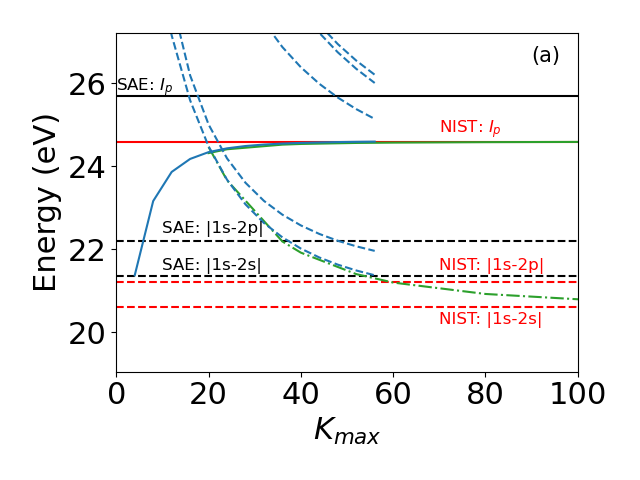
\includegraphics[width=0.49\linewidth]{figs/Two_electron/2nd_order_convergence.png}
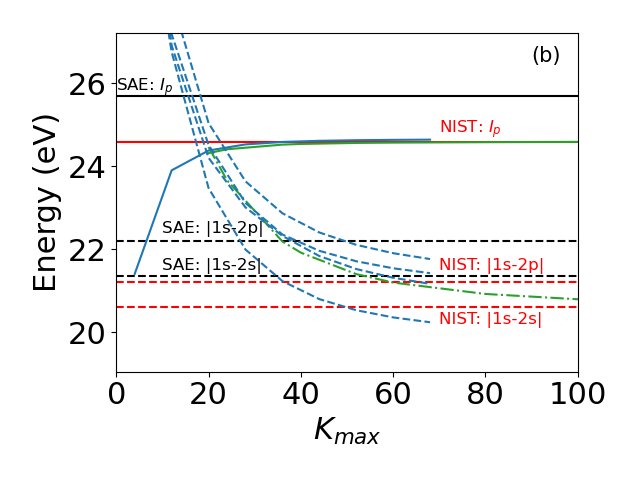
\includegraphics[width=0.49\linewidth]{figs/Two_electron/2nd_order_convergence_no_RRC.png}
\caption{Convergence of He atom first ionization potential (blue solid line) and excited states (blue dashed line) with RRC (left) and non-RRC (right) methods. Reference lines for He-SAE (black), NIST energies (red), and literature convergence (green, \cite{khan2015}) are shown.
} 
  \label{fig:he_2e_converg}
\end{figure}

To ensure the code is working properly, we have ran test on the convergences of the ionization potential and low lying bound states shown in Fig.~\ref{fig:he_2e_converg}. Panel (a) shows the convergence of the RRC method in blue as a function of the grand angular momentum using second order finite difference with a grid spacing of 0.05 au. The convergence is in good agreement with the green lines from a similar code \cite{khan2015}. Additionally, the NIST  (red) and SAE potential (black) energy levels are shown. Panel (b) shows the same data for the non-RRC method shown in blue. The non-RRC method has more low lying bound states that are due to not separating out the eigenstates with two spin up electrons. Taking account of it will reduce the runtime of the non-RRC method. As one can see, both methods produce highly accurate bound states quite quickly. The excited states, however, are slow to converge only outperforming the DFT based SAE potential energy levels with $K_{max} > 48$. As $K_{max}$ increases the matrix elements become increasingly difficult to calculate and the size of the wavefunction grows rapidly. This greatly limits the usefulness of this method for two electron calculations without the use of supercomputing resources.


\begin{figure}[!ht]
\centering
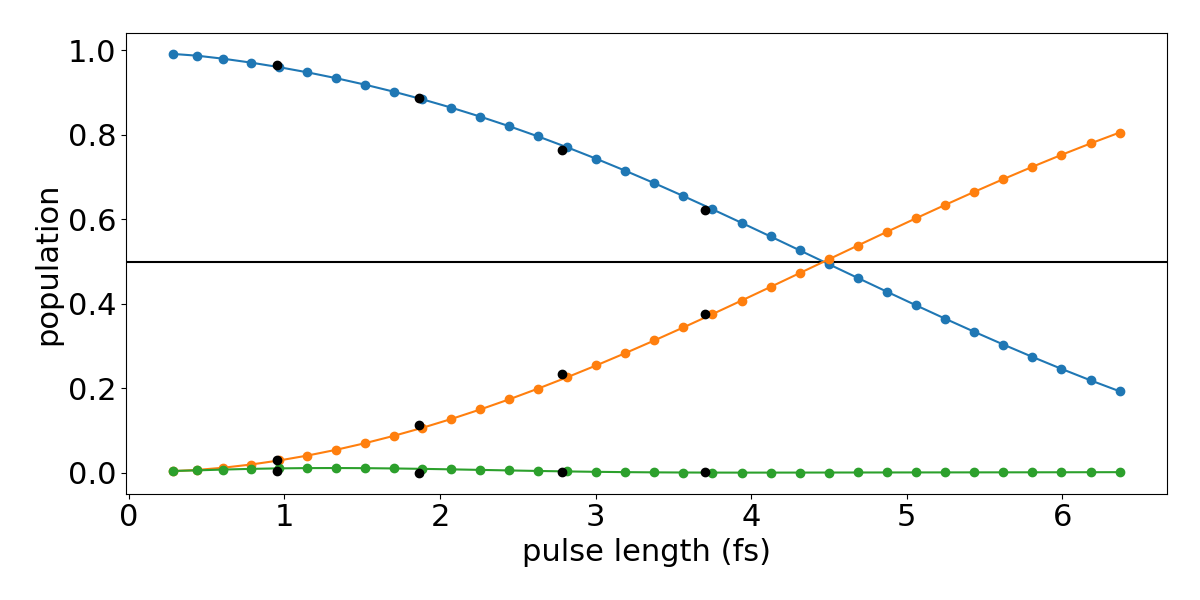
\includegraphics[width=\linewidth]{figs/Two_electron/1s-2p_rabi_flop_ee_sae.png}
\caption{Rabi flopping between the $1s$ and $2p$ states in helium atom. The populations in the $1s$ (blue), $2p$ (orange), and all other states (green) for the SAE code are plotted. The black dots show the two electrons simulations using the RRC method with $K_{max}=48$ agree well with the SAE results.
} 
  \label{fig:he_rabi_flop_ee}
\end{figure}

To test the stability and accuracy of the time propagation linearly polarized laser field, the RRC code was used to preform a $1s-2p$ Rabi flopping with $K_{max} = 48$ to closely match the $1s-2p$ energy gap to the SAE potential. The laser pulse had a sine squared envelope, peak intensity of $10^{14}$ W/cm$^2$, resonant central frequency of 0.812 au (0.822 au) for the SAE (RRC) code with varying pulse lengths ranging from 1 to 34 cycles. Fig.~\ref{fig:he_rabi_flop_ee} shows the SAE populations in the $1s$ (blue), $2p$ (orange), and all other bound/continuum states (green) for reference. The two electron populations are shown in black. The agreement is quite good, and the small discrepancy are due to slightly different energy gaps.
% section implementation_and_first_tests (end)

\section{Outlook} % (fold)
\label{sec:outlook}
The present methods still require improvement in order to perform converged two active electron simulations on desktop systems. Switching from the RRC to the non-RRC method lead to orders of magnitude reduction in runtime for matrix generation. However, the need to perform numerical integrals of Jacobi polynomials largely slows down the computation. Additionally, the slow convergence of excited states with respect to the grand angular momentum leads to large wavefuctions.  If the hyperangle $\alpha$ is discretized using finite difference, the integrals become integrals over delta functions and the slow convergence with respect to the grand angular momentum ($K$) may be avoided. 
% section outlook (end)
% chapter electron_correlation (end)